%Copyright 2014 Jean-Philippe Eisenbarth
%This program is free software: you can 
%redistribute it and/or modify it under the terms of the GNU General Public 
%License as published by the Free Software Foundation, either version 3 of the 
%License, or (at your option) any later version.
%This program is distributed in the hope that it will be useful,but WITHOUT ANY 
%WARRANTY; without even the implied warranty of MERCHANTABILITY or FITNESS FOR A 
%PARTICULAR PURPOSE. See the GNU General Public License for more details.
%You should have received a copy of the GNU General Public License along with 
%this program.  If not, see <http://www.gnu.org/licenses/>.

%Based on the code of Yiannis Lazarides
%http://tex.stackexchange.com/questions/42602/software-requirements-specification-with-latex
%http://tex.stackexchange.com/users/963/yiannis-lazarides
%Also based on the template of Karl E. Wiegers
%http://www.se.rit.edu/~emad/teaching/slides/srs_template_sep14.pdf
%http://karlwiegers.com


\documentclass{scrreprt}

\usepackage{pdfpages}
\usepackage{listings}
\usepackage[T1]{fontenc}
\usepackage{placeins}
\usepackage{float}
\usepackage{underscore}
\usepackage[bookmarks=true]{hyperref}
\usepackage[utf8]{inputenc}
\usepackage{graphicx}
\usepackage{subfigure}
\usepackage{xcolor,listings}
\usepackage[english]{babel}
\hypersetup{
	bookmarks=false,    % show bookmarks bar?
	pdftitle={Software Requirement Specification},    % title
	pdfauthor={Adam-Ryan},                     % author
	pdfsubject={TeX and LaTeX},                        % subject of the document
	pdfkeywords={TeX, LaTeX, graphics, images}, % list of keywords
	colorlinks=true,       % false: boxed links; true: colored links
	linkcolor=blue,       % color of internal links
	citecolor=black,       % color of links to bibliography
	filecolor=black,        % color of file links
	urlcolor=blue,        % color of external links
	linktoc=page            % only page is linked
}%
\def\myversion{1.0}
\date{}
%\title
\usepackage{hyperref}
\begin{document}
	
	\begin{flushright}
		\rule{16cm}{5pt}\vskip1cm
		\begin{bfseries}
			\Huge{Tutorial 2\\}
			\vspace{1.9cm}
			for\\
			\vspace{1.9cm}
			Data Mining - Transformation
			\vspace{1.9cm}
			\LARGE{Version \myversion}\\
			\vspace{1.9cm}
			Adam Ryan (14395076)\\
			\vspace{1.9cm}
			COMP47530\\
			\vspace{1.9cm}
			\today\\
		\end{bfseries}
	\end{flushright}
	
	\tableofcontents

	
\chapter{Question 1}
\section{Questions and answers}\label{E1Q}
Consider a dataset D that consists of customers purchasing tour packages to various places at different prices. We can perform different kinds of data operations on the dataset D. Try to
categorise the following operations into a) simple query of data retrieval, b) Online Analytical Processing, or c) Data Mining.

\begin{enumerate}
	\item Find names of customers who have purchased tours that cost less than €500.
	\begin{itemize}
		\item Simple Query of Data Retrieval. This is a standard query on a database selecting the distinct customer names filtered by tour price.
	\end{itemize}
	\item List the names of the customers, the number of tour packages that the customers have
	purchased, and the total cost for the tours.
	\begin{enumerate}
		\item OLAP. This requires rolling up tour-level data to customer level data, summing the tour costs and counting the distinct number of tour IDs for the customer.
	\end{enumerate}
	\item Calculate the difference in quarterly sales of tours between this year and the previous
	two years.
	\begin{itemize}
		\item OLAP. This requires rolling up tour sales by quarter by year (and may, depending on your approach, involve pivoting the data).
	\end{itemize}


	\item Find a rule such as "IF customers purchase a tour package to France, THEN it is 80\% likely
	that the same customers also purchase a tour package to Spain.
		\begin{itemize}
			\item Data Mining. The identification of an appropriate rule will involve the full data mining process as you are developing some form of rule-based model.
		\end{itemize}

	\item From the customer purchase history, build a model for predicting the kinds of customer who are likely to purchase tours to a certain country.

	\begin{itemize}
		\item Data Mining. The development of the model may be classified as data mining if the model is appropriately sophisticated to build out customer clusters and appropriately analyse the purchase history (of course, simplified models could be developed relying solely on OLAP such as a simple frequent travel and total payment segmentation model, but a 'proper' completion of the process will be data mining).
	\end{itemize}
\end{enumerate}

	
\newpage
\chapter{Question 2}
\section{Questions and Answers}
Consider the dataset given in DW\_Dataset.csv, representing the employee data of a company.


\begin{enumerate}
	\item If the attribute “Salary” needs to be discretised into three pay bands, suggest a simple yet sensible solution for the discretisation based with a valid argument.
		\begin{itemize}
			\item A simple way of banding the saleries based on the information provided would be categorise them as Low corresponding with under €2800, Medium corresponding with €2800 to €5600, and High corresponding with over 5600. The logic of this split would be based on splitting the total salary range in the data present into three groups. These groups appropriately capture Juniors into the lower tier (where we see there's a low standard deviation in salary between people in the same position), seniors into the medium range, and directors or executives into the high range. Using qcut or cut on the data results in ranges which fail to appropriately capture the key differentiator in salary (position). At lower levels, we see the salary is more concentrated with a lower deviation, while at higher levels (director) there is a larger salary deviation which suggests that the 'low' level should encompass a tighter band than upper bands, however we have limited information at the senior level to identify how varied salaries may be. As such, using the categorisation suggested keeps the low bracket small (as in reality the range is not 0 to 2800 but minimum wage to 2800), the medium range larger, and the high range unbounded.
		\end{itemize}
	\item Miss Davis's salary is unknown, and the unknown value needs to be imputed, what is a sensible replacement value and why?
		\begin{itemize}
		\item I would replace this with 3300 as we see she is a senior technician and based on the junior technician and director salaries we see that salaries broadly correlate to your level of experience.
		\end{itemize}
	
	\item Among the employee records, which record can be considered as an outlier? What harm can an outlier cause to the understanding of the dataset?
		\begin{itemize}
			\item I would classify Jones is an outlier in the dataset. There is a positive correlation between Age and Salary (explained via seniority) within the dataset, yet despite being 44 years old Jones is a Technician on a salary of 1800. This is a significant divergence from the other datapoints (the one point which might be considered an exception is Moore who, at 25, is a senior technician, however this is not as significant a divergence as Jones). We see this as an outlier when we plot the values:
				\begin{figure}[h!]
				\centering
				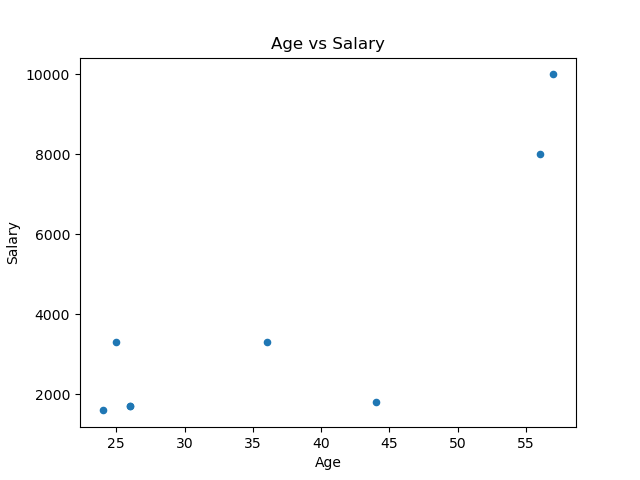
\includegraphics[width=0.4\linewidth]{age_outlier.png}
				\caption{Age vs Salary}\label{q2}
			\end{figure}
		\end{itemize}
\end{enumerate}
\noindent Online Analytical Processing (OLAP) perceives a dataset in a multi-dimensional space. For the dataset given in DW\_Dataset.csv, perform the following tasks/operations:
\begin{enumerate}
	\item[4.] Draw a diagram of a 3D view using the following attributes: Year of Birth, Status, and Salary.
\begin{itemize}
	\item I have created a 3D view using matplotlib, graphing Year of Birth, Status, and Salary. Please refer to figure \ref{q3}. 
	
	\begin{figure}[h!]
		\centering
		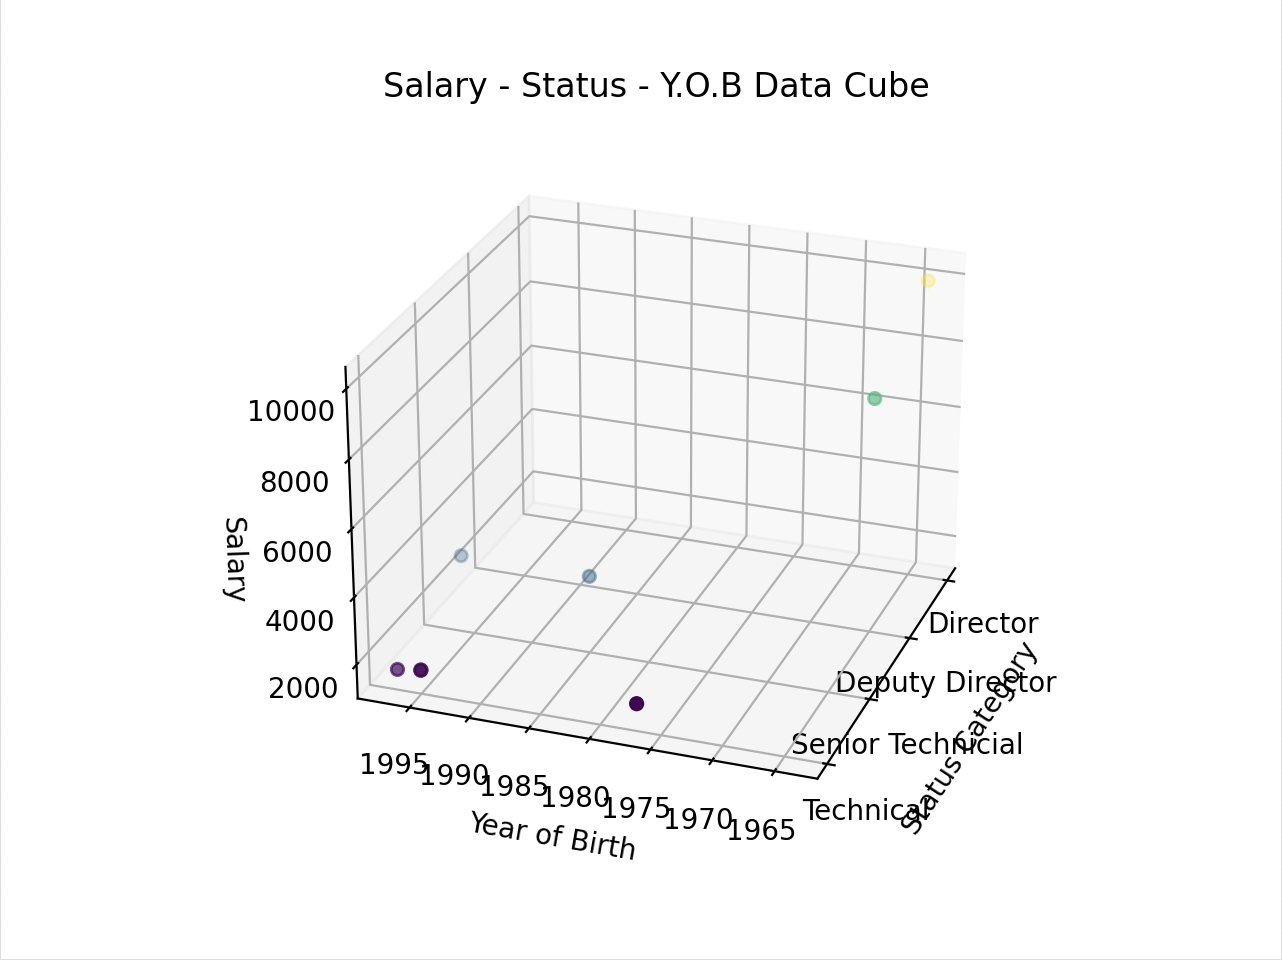
\includegraphics[width=0.95\linewidth]{3d_plot.png}
		\caption{3D View of Data}\label{q3}
	\end{figure}

\end{itemize}

	\item[5.] What do the data points inside the cube represent? Use the cube as an example to discuss the meaning of OLAP operations such as pivoting, slicing and dicing, rolling up and drilling down.
\begin{itemize}
	\item Each point represents a 3-dimensional vector such that the first element is an element of the set of values of Status, the second element is an element of the sest of values of Year of Birth, and the third element is an element of the set of values of Salary.
	\begin{itemize}
		\item Pivoting corresponds with rotating the cube for an alternative view of the data.
		\item Slicing and dicing corresponds with filtering dimensions of the cube. I.e. if one only wished for  the 'Status' attribute to correspond with 'Technician', Slicing would involve taking the plane of the cube which corresponds with this value, while dicing involves cutting the cube along multiple planes to extract a subcube, for example the sub-cube where 'Status'=Technician and 'Status' = 'Senior Technician'.
		\item Rolling up involves aggregating the data over a dimension e.g. finding the total salary by status.
		\item Drilling down involves subdividing the data into more granularity e.g. if we had Date of Birth instead of Year of birth, drilling down into this column might involve subdividing Date of Birth a more granular combination of Year, quarter, Month, or Day of Birth or the day number of date of birth  since 1900.
	\end{itemize}
\end{itemize}

\end{enumerate}

\newpage
\chapter{Question 3}
\section{Questions and Answers}

Suppose that a data warehouse for Big University consists of the four dimensions student, course, semester, and instructor, and two measures count and avg\_grade. At the lowest conceptual level (e.g., for a given student, course, semester, and instructor combination), the avg\_grade measure stores the actual course grade of the student. At higher conceptual levels, avg\_grade stores the average grade for the given combination.

\begin{enumerate}
	\item Draw a snowflake schema diagram for the data warehouse.
		\begin{itemize}
			\item  I've created a high-level schema for big university focusing on four required dimensions, with a few optional dimension tables. In particular, to a student I've added on address (which itself has county and country references) to store the student's term address, registration status (as it's referred to in the question below), the degree major and the degree. To an instructor, I've added on their position (Assistant Lecturer, Lecturer, Associate Professor, etc.). To the semester I've added on the year of the semester.
				\begin{figure}[h!]
				\centering
				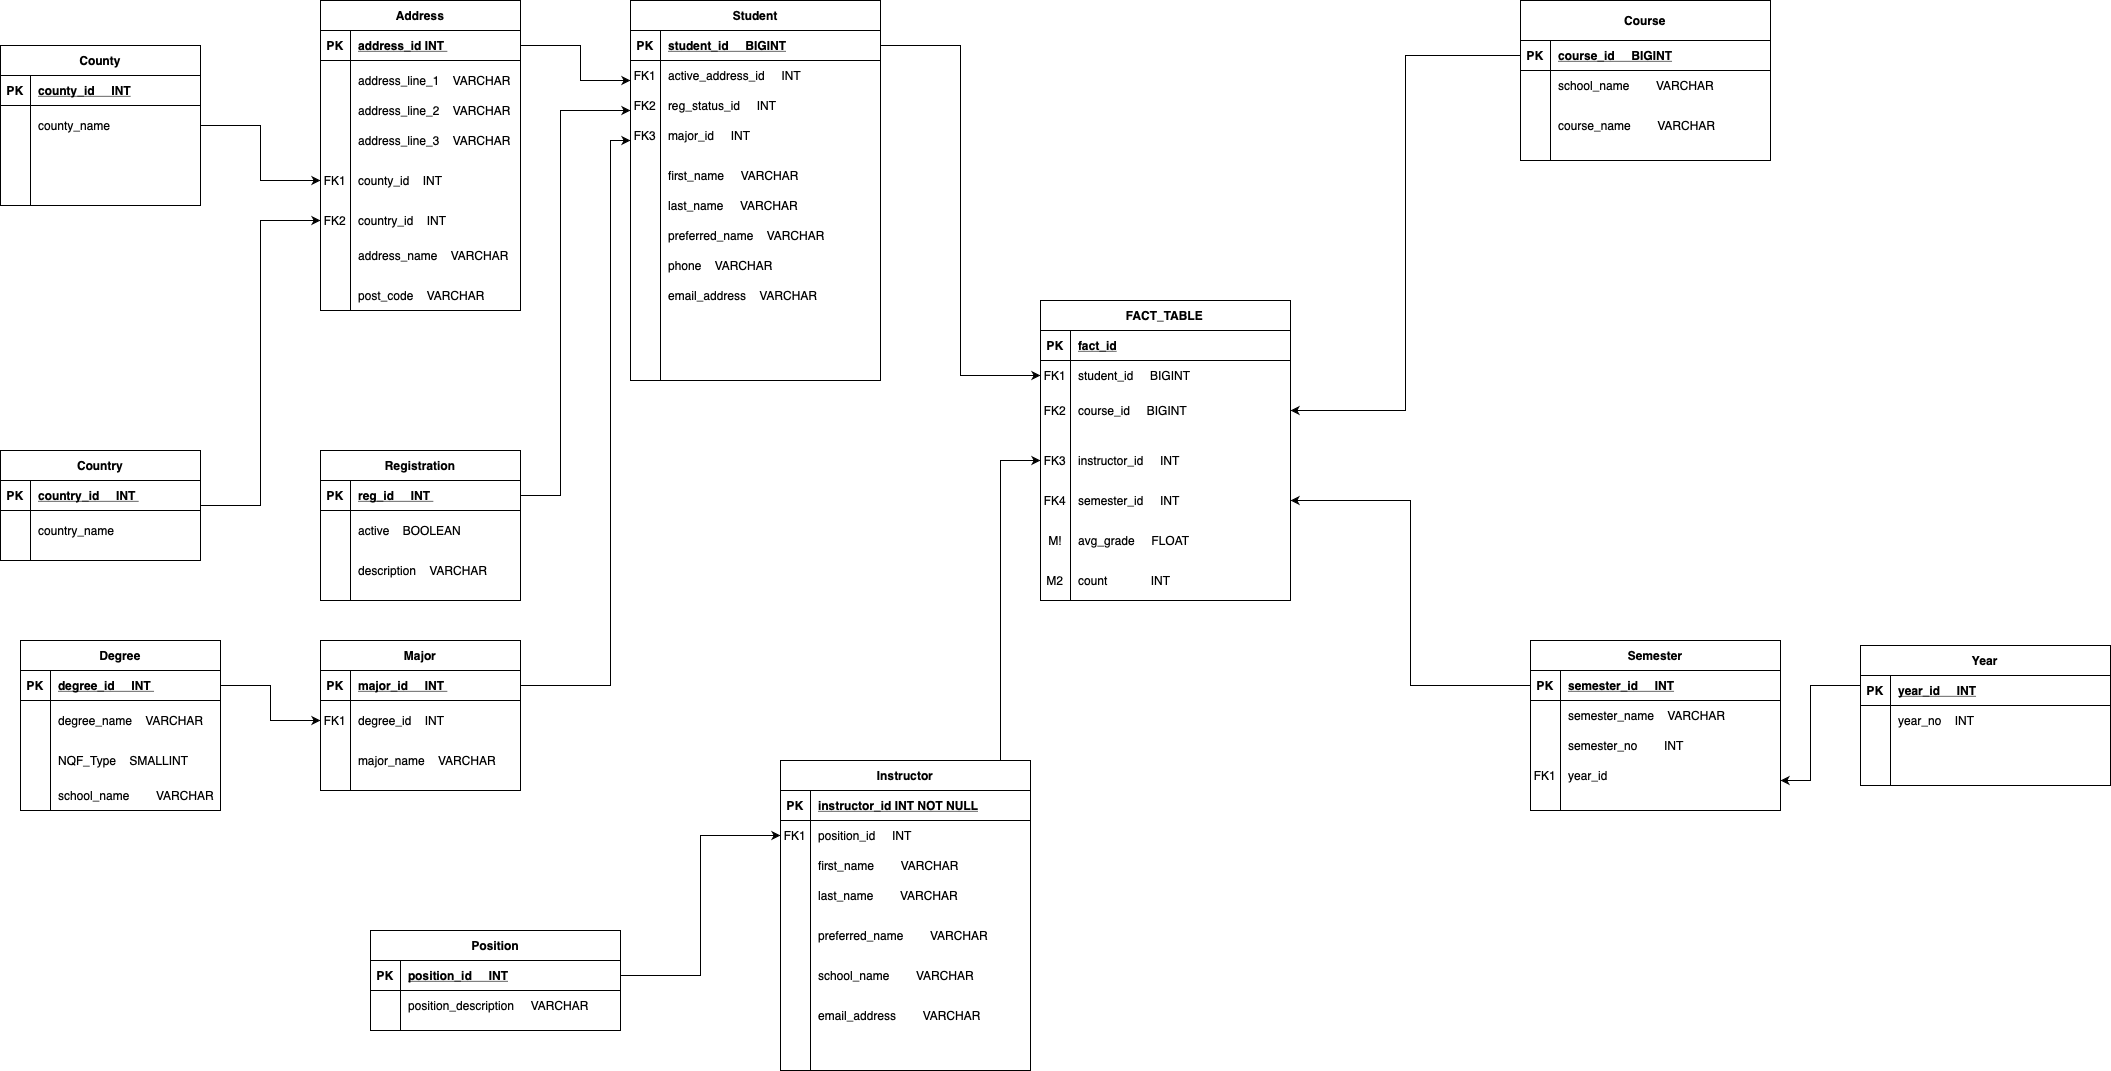
\includegraphics[width=0.95\linewidth]{DataMining.drawio.png}
				\caption{BigUniversity Schema}\label{q3}
			\end{figure}
		\end{itemize}
	
	\item Starting with the base cuboid [student, course, semester, instructor], what specific OLAP operations (e.g., roll-up from semester to year) should you perform to list the average grade of CS courses for each Big University student.
\begin{itemize}
	\item Note, I am assuming it is looking for the student's average grade across ALL computer science courses. I.e. That it is not asking about course PER student. The specific OLAP operations are:
		\begin{itemize}
			\item Roll up course to school name of CS.
			\item Dice where course's school name is CS
			\item Drill across to student first name and last name.
			\item Take the average grade grouped by student.
		\end{itemize}
	\item Specifically, you're taking the avg grade grouped by student from the table where the courses are inner joined on the course table where school name is CS.
	\item An MSSQL query to accomplish this would be:
	\begin{lstlisting}[
		language=SQL,
		showspaces=false,
		basicstyle=\ttfamily,
		numbers=left,
		numberstyle=\tiny,
		commentstyle=\color{gray}
		]
		SELECT
			s.student_id					AS		[Student ID]
			,s.first_name					AS 		[First Name]
			,s.last_name					AS		[Last Name]
			,AVG(ft.avg_grade)			AS		[Grade]
		FROM
			(SELECT
				course_id
			FROM
				course
			WHERE
				school_name='CS') cs
			
		INNER JOIN
			fact_table ft
		ON
			cs.course_id=ft.course_id
			
		INNER JOIN
			(SELECT
				st.student_id
				,st.first_name
				,st.last_name
			FROM
				student st
			) s
		ON
			s.student_id=ft.student_id
			
		GROUP BY
			s.student_id
			,s.first_name
			,s.last_name
	\end{lstlisting}
	\item If instead you are looking for the average grade per student per course where course is CS, then you do the exact same as above except you group by course\_id and drill across to course name as well.
	\item I am assuming university is BigUniversity for all students and courses as this is stated in the question.
\end{itemize}
	\item  If each dimension has five levels (including all), such as “student < major < status < university < all”, how many cuboids will this cube contain (including the base and apex cuboids)?
\begin{itemize}
		\item We have 4 dimensions and each dimension has 5 levels, therefore we have $5^4 = 625$ cuboids.
\end{itemize}

\end{enumerate}

\noindent The following questions will guide you to implement a data warehouse using PostgreSQL. At this stage, we assume that you have already defined the DW schema, with subjects, dimensions, and measures.

\begin{enumerate}
	\item[4.] First, you need to establish a connection with the database to create a table where you can store records and arrays of data. Make sure you follow the PostgreSQL naming convention.
\begin{itemize}
	\item Done. I've named the table input\_dw\_data with columns: [id, first\_name, middle\_name, last\_name, favourite\_number, location]
\end{itemize}
	\item[5.] Second, you need to create another connection to the DW where you will store your datasets in.
\begin{itemize}
	\item Done.
\end{itemize}

	\item[6.] Create a data file that contains 5 entries, called “input\_DW\_data.csv”, which you need to store in your DW.
\begin{itemize}
	\item Done
\end{itemize}

	\item[7.] Finally, you need to define the following functions to read, write, update, and list your data to / from the data warehouse.
	\\
	\\
	def read\_record (field, name, engine): ...
	\\
	def write\_record (name, details, engine): ...
	\\
	def update\_record (field name, new value, engine):  ...
	\\
	def read\_dataset (name, engine):  ...
	\\
	def write\_dataset (name, dataset, engine):  ...
	\\
	def list\_datasets (engine):  ...
\begin{itemize}
	\item Note, I have created functions which accomplish this however, the functions which are here are poorly defined; how general are the functions expected to be, which tables should they operate on, what columns should they work with, what are the meanings of the inputs, etc. As such, in defining these functions I have kept them highly general, however to do this I have had to alter what inputs are present. For example, my functions will allow a user to read and write to any table in any database, update any column against any record in any table, etc. and protects against sql injection using psycopg2 and it's union functions to allow for a Dynamic SQL alternative. However, because the question has not defined the database requirements this may require modification for a demonstrator to run. As such, I have copied a full output of what this function looks like below because I cannot guarantee it will work for the demonstrator without proper configuration which was not provided.
\begin{lstlisting}
	Write Dataset:
	
	Read Dataset:
	
	id first_name middle_name last_name  favourite_number        location
	0   1       Adam     Patrick      Ryan                 7         Ireland
	1   2        Joe       Jemma     Smith                 4         Ireland
	2   3      Peter       Paris  Petigrew                 7  United Kingdom
	3   4        Fav           u     Orite                 8           Spain
	4   5       Jill       Gilly  Gilligan                 1         Ireland
	Insert:
	
	id first_name middle_name last_name  favourite_number        location
	0   1       Adam     Patrick      Ryan                 7         Ireland
	1   2        Joe       Jemma     Smith                 4         Ireland
	2   3      Peter       Paris  Petigrew                 7  United Kingdom
	3   4        Fav           u     Orite                 8           Spain
	4   5       Jill       Gilly  Gilligan                 1         Ireland
	5   6        New      Sample      Data                 6         Ireland
	Reading Record:
	
	
	id:6
	
	
	first_name:New
	
	
	middle_name:Sample
	
	
	last_name:Data
	
	
	favourite_number:6
	
	
	location:Ireland
	
	Updating Record:
	
	Read Dataset After update:
	
	id first_name middle_name last_name  favourite_number        location
	0   1       Adam     Patrick      Ryan                 7         Ireland
	1   2        Joe       Jemma     Smith                 4         Ireland
	2   3      Peter       Paris  Petigrew                 7  United Kingdom
	3   4        Fav           u     Orite                 8           Spain
	4   5       Jill       Gilly  Gilligan                 1         Ireland
	5   6        New      Sample      Data                 6  UpdateLocation
	
	Out[92]:
	
	{'input_dw_data':    id first_name middle_name last_name  favourite_number        location
		0   1       Adam     Patrick      Ryan                 7         Ireland
		1   2        Joe       Jemma     Smith                 4         Ireland
		2   3      Peter       Paris  Petigrew                 7  United Kingdom
		3   4        Fav           u     Orite                 8           Spain
		4   5       Jill       Gilly  Gilligan                 1         Ireland
		5   6        New      Sample      Data                 6  UpdateLocation}
\end{lstlisting}
\end{itemize}
%
%	\item 
%\begin{itemize}
%	\item 
%\end{itemize}
%
%	\item 
%\begin{itemize}
%	\item 
%\end{itemize}
%
%	\item 
%\begin{itemize}
%	\item 
%\end{itemize}
%
%	\item 
%\begin{itemize}
%	\item 
%\end{itemize}	

\end{enumerate}
	
\end{document}
